\subsection{Láthatóság, árnyalás, megvilágítás, színmodellek, anyagmodellek.}

\textbf{Megjelenési algoritmusok – láthatóság:}
\begin{itemize}
    \item lényegük, hogy el lehessen dönteni, hogy egy adott nézőpontból melyik objektum látszódik egy adott helyen (pixelenként)
    \item \textbf{Depth Sort algoritmus}
    \begin{itemize}
        \item a háromszögekkel közelített felület elemei a legtávolabbi pontjaik szerint sorba rendezve
        \item jó a két összehasonlított háromszög sorrendja, ha
        \begin{itemize}
            \item az „a” háromszög legtávolabbi pontja közelebb van a képsíkhoz, mint. a „b” háromszög legközelebbi pontja
            \item a befoglaló téglalapok nem metszik egymást
            \item az „a” háromszög vetített képe nem metszi „b” háromszög vetített képét
            \item a „b” háromszög mindhárom pontja az „a” háromszög síkja mögött helyezkedik el
        \end{itemize}
        \item egyébként csere
    \end{itemize}
    \item \textbf{Area subdivision:}
    \begin{itemize}
        \item takarás vizsgálata raszteres szemlélettel
        \item a képernyőt 1 részre osztjuk
        \item tudjuk, hogy a térnegyedben melyik háromszög látszik, ha
        \begin{itemize}
            \item az ablakot egyetlen háromszög foglalja be
            \item egyetlen háromszög sincs az ablakban
            \item az ablak egyetlen háromszöget metsz, vagy foglal magában
            \item valamelyik háromszögről tudjuk, hogy takar
        \end{itemize}
        \item a negyedeket további négy részre osztva folytatható pixelméretig
    \end{itemize}
    \begin{center}
        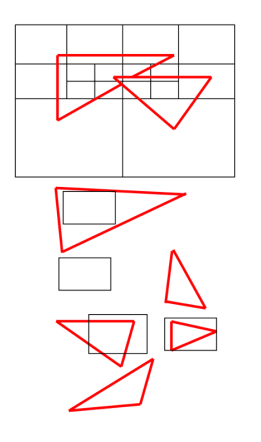
\includegraphics[width=0.6\textwidth]{res/imgs/info_23_area_subdivision.png}
    \end{center}
    \item \textbf{Z-puffer:}
    \begin{itemize}
        \item minden pixelre mélység számítása
        \item ha az érték kisebb, mint ami a Z-pufferben szerepel -» kirajzoljuk, amúgy nem
    \end{itemize}
    \begin{center}
        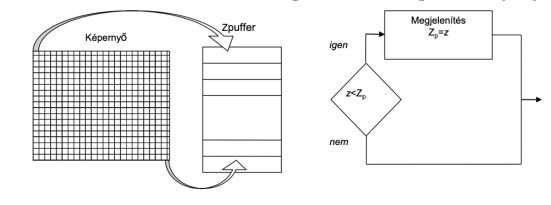
\includegraphics[width=0.8\textwidth]{res/imgs/info_23_z_buffer.png}
    \end{center}
\end{itemize}

\begin{center}
    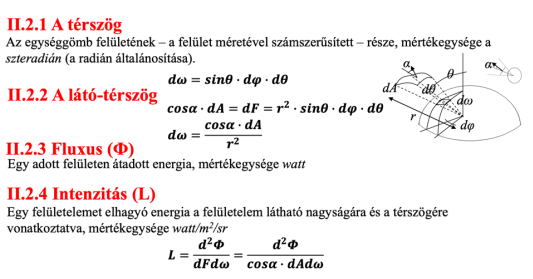
\includegraphics[width=0.95\textwidth]{res/imgs/info_23_solid_angle.png}
\end{center}

\textbf{Árnyalás:}
\begin{itemize}
    \item visszaverődési sűrűségfüggvény
    \begin{itemize}
        \item $w(\omega, x, \omega')$
        \item $w(\omega, x, \omega') d\omega = P(\text{a foton } \omega \text{ irányban } d\omega\text{-ban megy | } \omega' \text{ irányból, } d\omega'\text{-n belülről})$
    \end{itemize}
    \item \textbf{BRDF}
    \begin{itemize}
        \item kétirányú visszaverődés-eloszlási függvény -- Bidirectional Reflection Distributon Function
    \end{itemize}
\end{itemize}
\begin{center}
    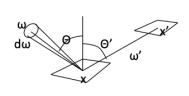
\includegraphics[width=0.7\textwidth]{res/imgs/info_23_brdf.png}
\end{center}

\textbf{Megvilágítás:}
\begin{center}
    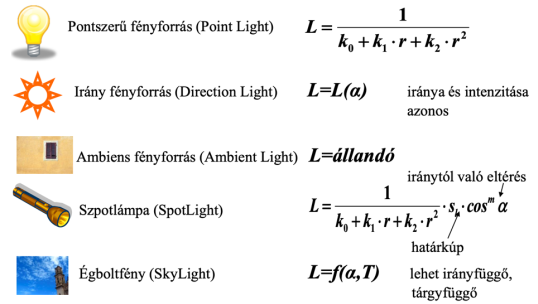
\includegraphics[width=0.95\textwidth]{res/imgs/info_23_lighting_types.png}
\end{center}

\textbf{Színmodellek:}
\begin{center}
    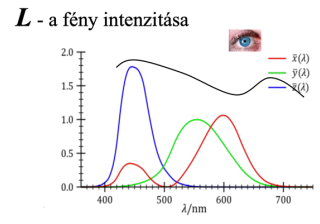
\includegraphics[width=0.95\textwidth]{res/imgs/info_23_color_models.png}
\end{center}
\begin{itemize}
    \item színdefiníció
    \begin{itemize}
        \item fekete -- fehér: 0,1
        \item szürke árnyalat: 0-255
        \item színes (RGB, RGBA, CMYK, HLS)
    \end{itemize}
\end{itemize}

\textbf{Anyagmodellek:}
\begin{itemize}
    \item \textbf{diffúz anyagok:} minden irányban egyenletes -- Lambert törvény
    \begin{equation*}
        L^R = L^{in} \cdot k_{d,\lambda} \cdot \cos(\theta')
    \end{equation*}
    \begin{minipage}{0.4\textwidth}
        \begin{center}
            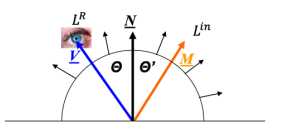
\includegraphics[width=\textwidth]{res/imgs/info_23_diffuse_vectors.png}
        \end{center}
    \end{minipage}
    \hfill
    \begin{minipage}{0.4\textwidth}
        \begin{center}
            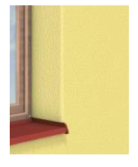
\includegraphics[width=0.4\textwidth]{res/imgs/info_23_diffuse_image.png}
        \end{center}
    \end{minipage}

    \item \textbf{reflexív anyagok:} ideális visszaverődés -- pl. tükör
    \begin{equation*}
        L^R = L^{in} \cdot k_{r,\lambda} \cdot \delta_{\theta = \theta'}
    \end{equation*}
    \begin{minipage}{0.4\textwidth}
        \begin{center}
            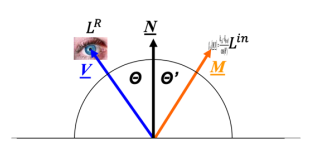
\includegraphics[width=\textwidth]{res/imgs/info_23_reflective_vectors.png}
        \end{center}
    \end{minipage}
    \hfill
    \begin{minipage}{0.4\textwidth}
        \begin{center}
            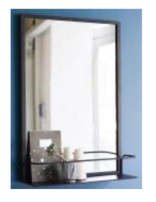
\includegraphics[width=0.4\textwidth]{res/imgs/info_23_reflective_image.png}
        \end{center}
    \end{minipage}

    \item \textbf{ideális fénytörés} -- pl. üveg
    \begin{equation*}
        L^R = L^{in} \cdot k_{t,\lambda} \cdot \delta_{\theta = \theta_T}
    \end{equation*}
    \begin{center}
        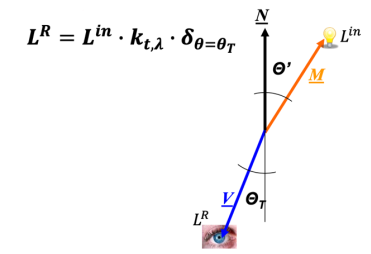
\includegraphics[width=0.4\textwidth]{res/imgs/info_23_refractive_vectors.png}
    \end{center}

    \item \textbf{Spekuláris visszaverődés:} csak a visszaverődés környékén -- Phong modell -- pl. CD
    \begin{equation*}
        L^R = L^{in} \cdot k_{s,\lambda} \cdot \cos^n(\psi)
    \end{equation*}
    \begin{minipage}{0.4\textwidth}
        \begin{center}
            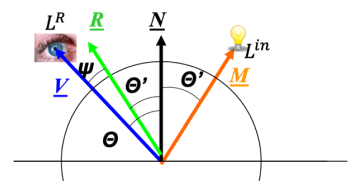
\includegraphics[width=\textwidth]{res/imgs/info_23_specular_vectors.png}
        \end{center}
    \end{minipage}
    \hfill
    \begin{minipage}{0.4\textwidth}
        \begin{center}
            
\includegraphics[width=0.4\textwidth]{res/imgs/info_23_specular_image.png}
        \end{center}
    \end{minipage}
\end{itemize}